\documentclass[12pt,fleqn]{beamer}
\usepackage{verbatim}


\xdefinecolor{lavendar}{rgb}{0.8,0.6,1}
\xdefinecolor{olive}{cmyk}{0.64,0,0.95,0.4}
%\xdefinecolor{olive}{cmyk}{1,0,0,0}
\xdefinecolor{mag}{cmyk}{0.1,1,0,0.2}
\xdefinecolor{lblue}{rgb}{0,0,1.5}
\xdefinecolor{lred}{rgb}{1,0,0}
\xdefinecolor{mine}{cmyk}{1,0,0.2,0}
\xdefinecolor{bluel}{cmyk}{0.1,0,0.9,0.4}

\usepackage{amsmath,amssymb,dsfont,mathrsfs}
\usepackage{tikz,pgflibraryplotmarks}
\usepackage{multimedia}
\usepackage{wasysym}
\usepackage{rotating}
\usepackage{algorithm,algorithmic}
\usepackage{graphicx} % more modern
\usepackage{subfigure}
\usepackage{booktabs}

\usepackage{pgfplots}
\usepackage{verbatim}

\usepackage{setspace}
\newlength\iwidth
\newlength\iheight

\newcommand\makebeamertitle{\frame{\maketitle}}%
\graphicspath{{./images/}}
\setbeamertemplate{navigation symbols}{}
\addtobeamertemplate{navigation symbols}{}{%
    \usebeamerfont{footline}%
    \usebeamercolor[fg]{footline}%
	\insertshorttitle
    \;--
    \insertframenumber
}

\newcommand{\sectionstart}{
	\only<beamer>{
 	\begin{frame}% (fold)
 		\begin{centering}\Huge \insertsection \par\end{centering}
 	\end{frame}% frame the_application (end)
	}
 }


% make bibliography entries smaller
\usepackage{natbib}
\setbeamertemplate{bibliography item}{[\theenumiv]}
\renewcommand\bibfont{\scriptsize}
\setbeamertemplate{frametitle continuation}[from second]
\newcommand{\tcr}{\textcolor{red}}
\newcommand{\tcrd}{\textcolor{red}}
\newcommand{\tcb}{\textcolor{bluel}}
\newcommand{\tcm}{\textcolor{mag}}
\newcommand{\tcg}{\textcolor{olive}}

\newcommand{\R}{\mathbb{R}}
\newcommand{\C}{\mathbb{C}}

% bold lower-case for vectors
\newcommand{\bfa}{{\bf a}}
\newcommand{\bfb}{{\bf b}}
\newcommand{\bfc}{{\bf c}}
\newcommand{\bfs}{{\bf s}}
\newcommand{\bfm}{{\bf m}}
\newcommand{\bfd}{{\bf d}}
\newcommand{\bfe}{{\bf e}}
\newcommand{\bfu}{{\bf u}}
\newcommand{\bfy}{{\bf y}}
\newcommand{\bfx}{{\bf x}}
\newcommand{\bfh}{{\bf h}}
\newcommand{\bfw}{{\bf w}}
\newcommand{\bfv}{{\bf v}}
\newcommand{\bfr}{{\bf r}}
\newcommand{\bfz}{{\bf z}}
\newcommand{\bfp}{{\bf p}}


% bold upper-case for linear operators
\newcommand{\bfA}{{\bf A}}
\newcommand{\bfB}{{\bf B}}
\newcommand{\bfZ}{{\bf Z}}
\newcommand{\bfM}{{\bf M}}
\newcommand{\bfC}{{\bf C}}
\newcommand{\bfD}{{\bf D}}
\newcommand{\bfQ}{{\bf Q}}
\newcommand{\bfJ}{{\bf J}}
\newcommand{\bfG}{{\bf G}}
\newcommand{\bfI}{{\bf I}}
\newcommand{\bfP}{{\bf P}}
\newcommand{\bfK}{{\bf K}}
\newcommand{\bfY}{{\bf Y}}
\newcommand{\bfW}{{\bf W}}
\newcommand{\bfR}{{\bf R}}
\newcommand{\bfL}{{\bf L}}
\newcommand{\bfF}{{\bf F}}
\newcommand{\bfT}{{\bf T}}
\newcommand{\bfS}{{\bf S}}
\newcommand{\bfX}{{\bf X}}
\newcommand{\bfU}{{\bf U}}
\newcommand{\bfV}{{\bf V}}
\newcommand{\bfH}{{\bf H}}


\newcommand{\calF}{\mathcal{F}}



\newcommand{\hf}{{\frac 12}}
\newcommand{\bftheta}{{\boldsymbol \theta}}
\newcommand{\bfxi}{{\boldsymbol \xi}}

\newcommand{\bfLambda}{{\boldsymbol \Lambda}}
\newcommand{\bfSigma}{{\boldsymbol \Sigma}}
\newcommand{\bfepsilon}{{\boldsymbol \epsilon}}

\newcommand{\E}{\vec E}
\newcommand{\B}{\vec B}

\newcommand{\vu}{  {\vec {\bf u}}}

\newcommand{\grad}{  {\vec {\bf \nabla}}}

\newcommand{\lfrownie}{\textcolor{red}{\large{\frownie}}}
\newcommand{\lsmiley}{\textcolor{green}{\large{\smiley}}}

\newcommand{\curl}{\ensuremath{\nabla\times\,}}
\renewcommand{\div}{\nabla\cdot\,}
\newcommand{\divh}{\nabla_h\cdot\,}
\renewcommand{\grad}{\ensuremath{\nabla}}

\DeclareMathOperator*{\argmin}{arg\,min}


\title[Iterative LS]{Solving the Least-Squares Problem in Practice}
\subtitle{Numerical Methods for Deep Learning}
\date{}

\begin{document}

\makebeamertitle

% section bias_variance (end)

\section{Iterative Methods} % (fold)
\label{sec:iterative_methods}
\begin{frame}\frametitle{Iterative Solvers for Least-Squares Regression}
	Last time: Given $\bfY\in \R^{n_f\times n}$ and $\bfC\in\R^{n_c\times n}$, solve
	$$
	\min_{\bfX}  \frac12\left\|  \bfA   \bfX  -  \bfC^\top \right\|_F^2
	$$
	directly using $\bfX^* = (\bfA^{\top} \bfA)^{-1}\bfA^{\top} \bfC^\top$. Here
	$$
		\bfA = \begin{pmatrix}
			\bfY^\top && \bfe_n
		\end{pmatrix}, \quad \text{ and } \quad 
		\bfX = \bfW^\top \in \R^{(n_f+1)\times n_c}.
	$$
	Problems: Generating  $\bfA^{\top}\bfA$ and solving normal equations is too costly for large-scale problems.
	
	\pause

	\bigskip
	
Today: Iterative methods that avoid working with $\bfA^{\top}\bfA$ 
\begin{itemize}
\item Steepest descent 
\item Conjugate gradient for least-squares (CGLS)
\end{itemize}
Excellent references: Numerical Optimization~\cite{NocedalWright2006}, iterative linear algebra~\cite{Saad2003}, general introduction \cite{AscherGreif2011}
\end{frame}

\begin{frame}\frametitle{Iterative Methods}


General idea - obtain a sequence $\bfX_1, \ldots,\bfX_j,\ldots$
that converges to least-squares solution $\bfX^*$

$$
	\bfX_j \longrightarrow \bfX^*, \quad \text{ for } \quad j \to \infty.
$$

\bigskip

How fast does the sequence converge? Assume
$$
\|\bfX_{j+1} - \bfX^* \| < \gamma_j \|\bfX_{j} - \bfX^* \|
$$ 
where all $\gamma_j < 1$. Then

\begin{itemize}
\item If $\gamma_j$ is bounded away from $0$ and 1 the convergence is linear
\item If $\gamma_j \rightarrow 0$ the convergence is superlinear
\item If $\gamma_j \rightarrow 1$ the convergence is sublinear
\end{itemize}

The sequence converges quadratically if $\gamma_j$ is bounded away from 0 and 1 and 
$$ \|\bfX_{j+1} - \bfX^* \| < \gamma_j \|\bfX_{j} - \bfX^* \|^2 $$ 
\end{frame}


\begin{frame}
	\frametitle{Steepest Descent}
	Most basic iterative technique for solving $\min_\bfx \phi(\bfx)$
	\begin{center}
		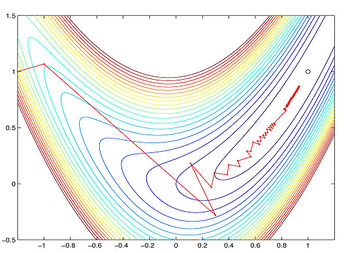
\includegraphics[width=6cm]{steepestDescent.jpg}
	\end{center}
	\begin{equation*}
		\bfx_{j+1} = \bfx_j + \alpha_j \bfd_j \quad \text{ with } \quad \bfd_j =  - \nabla \phi(\bfx_j).
	\end{equation*}
	\pause
	Interpretation 1: $\bfd_{j+1}$ maximizes local descent, i.e., solves
	\begin{equation*}
		\min_{s} \phi(\bfx_j) + \bfd^\top \nabla \phi(\bfx_j) \quad \text{ subject to }\quad \|\bfd\|_2 = 1.
	\end{equation*}
	
	\pause
	
	Interpretation 2: $\bfd_j$ is orthogonal to level sets of $\phi$ at $\bfx_j$.
	
	
\end{frame}

\begin{frame}\frametitle{Steepest Descent for Least-Squares}

Consider now
$$ \phi(\bfx) = \hf \|\bfA \bfx - \bfc\|^2 \quad \text{ with } \quad \grad_{\bfx} \phi(\bfx) = \bfA^{\top}(\bfA \bfx -  \bfc).$$

\bigskip

Steepest descent direction is  $\bfd_j = \bfA^{\top}(\bfc - \bfA \bfx_j)$ and
$$ \bfx_{j+1} = \bfx_j + \alpha_j \bfd_j $$

How to choose $\alpha_j$? 
\pause
Idea: Minimize $\phi$ along direction $\bfd_j$
$$ 
\alpha_j = \argmin_\alpha \phi(\bfx_j + \alpha \bfd_j) = 
 \argmin_\alpha \hf \|\alpha \bfA \bfd_j - \bfr_j\|^2
$$
with residual $\bfr_j = \bfc - \bfA \bfx_j $.

\bigskip
\pause

This leads to simple quadratic equation in 1D whose solution is
 
  
$$ \alpha_j = {\frac { \bfr_j^{\top}\bfA\bfd_j}{\|\bfA \bfd_j\|^2}} $$


\end{frame}


\begin{frame}\frametitle{Algorithm: Steepest Descent for Least-Squares}


for $j=1,\ldots $
\begin{itemize}
\item Compute residual $\bfr_j = \bfc - \bfA \bfx_j$
\item Compute the SD direction $\bfd_j = \bfA^{\top}\bfr_j$
\item Compute step size  $\alpha_j = {\frac { \bfr_j^{\top}\bfA\bfd_j }{\|\bfA \bfd_j\|^2}}$
\item Take the step $\bfx_{j+1} = \bfx_j + \alpha_j \bfd_j$
\end{itemize}

\pause

Converges linearly, i.e., 
$$
	\| \bfX_{j+1} - \bfX^*\| < \gamma \|\bfX_j - \bfX^* \| \quad \text{ with } \quad \gamma \approx \left| {\frac {\kappa-1}{\kappa+1}} \right|
$$

Here, $\kappa$ depends on condition number of $\bfA$, i.e., 
$$ \kappa \approx {\frac {\sigma_{\bf min}^2}{\sigma_{\bf max}^2}} $$


Can be painfully slow for ill-conditioned problems

\end{frame}


\begin{frame}\frametitle{Accelerating Steepest Descent: Post-Conditioning}

\begin{columns}
	\column{.7\textwidth}
	
	Idea: Improve convergence by transforming the problem
	 $$ \phi(\bfx) = \hf \|\bfA \bfS \bfS^{-1}\bfx - \bfc \|^2$$
	
	Here: $\bfS$ is invertible

	Solve in two steps:
	\begin{enumerate}
		\item Set $\bfz = \bfS^{-1}\bfx$ and compute
	 $$ \bfz^* \argmin_{\bfz} \hf \|\bfA \bfS \bfz - \bfc \|^2$$
	 	\item Then $\bfx = \bfS \bfz$.
	\end{enumerate} 

	 \bigskip

	 Pick $\bfS$ such that $\bfA \bfS$ is better conditioned.

	\column{.3\textwidth}
	\pause
	\begin{tabular}{@{}c@{}}
		original problem: \\
		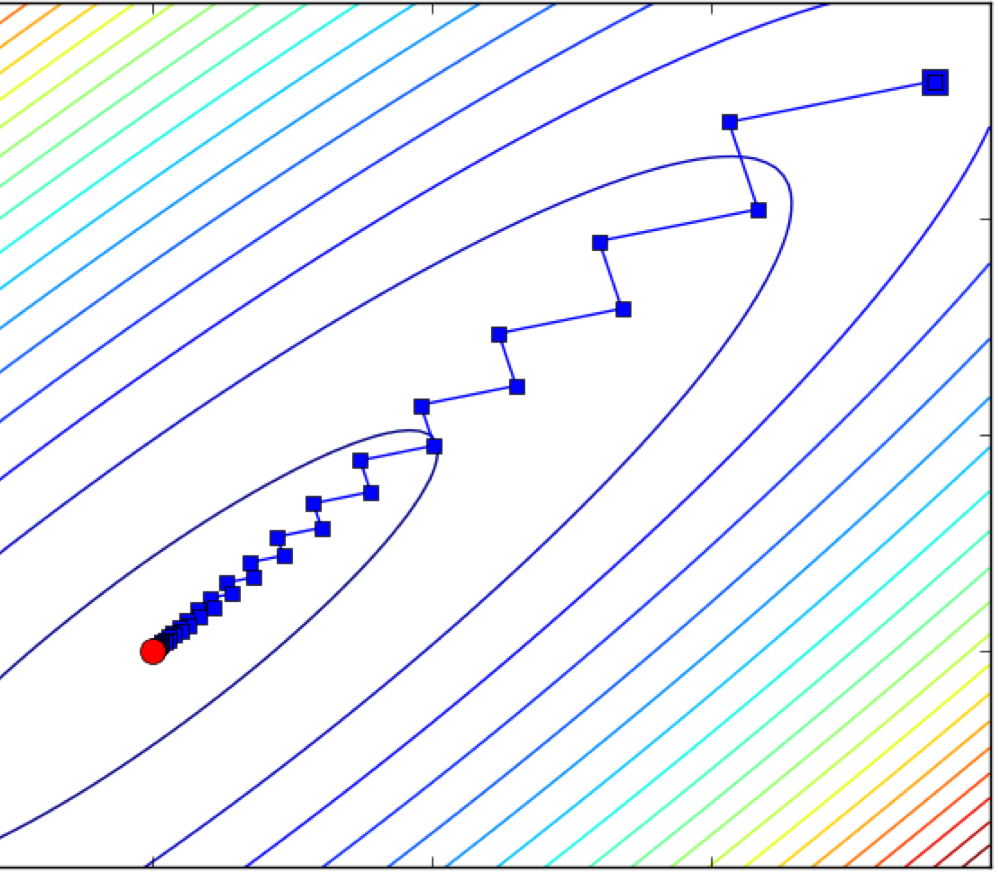
\includegraphics[width=35mm]{convSD2DQuadratic}\\
		post-conditioned:\\
		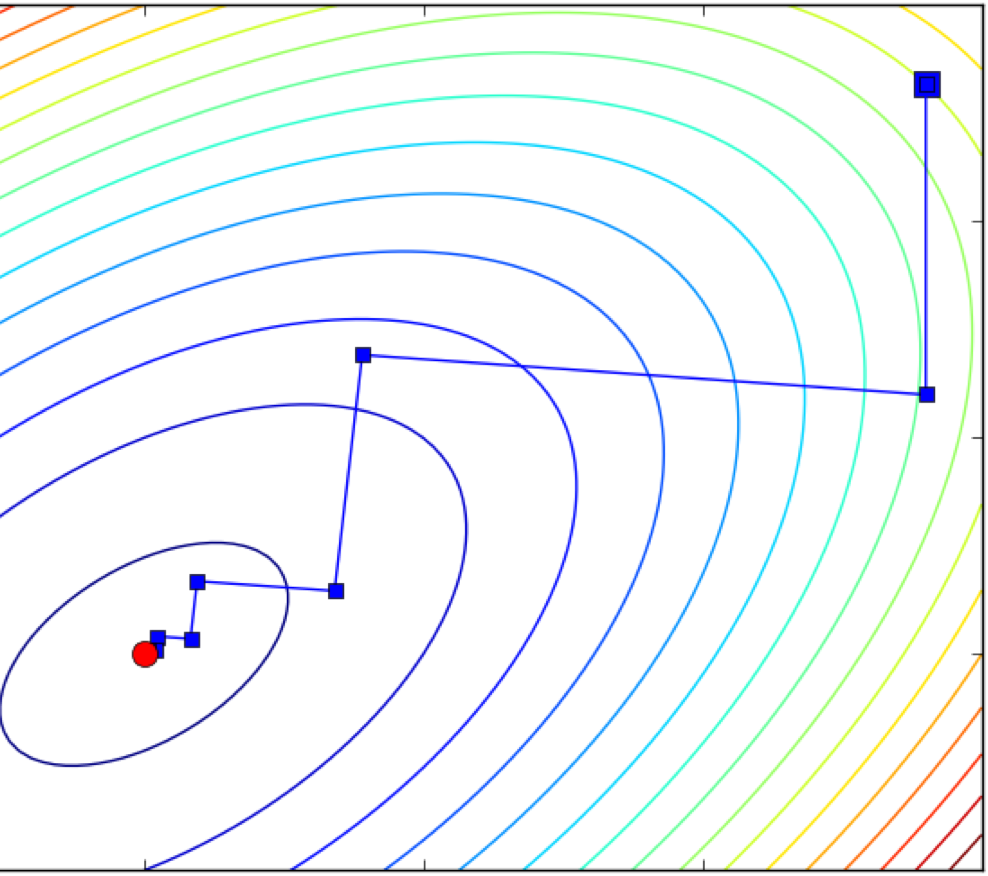
\includegraphics[width=35mm]{convSD2DQuadraticGood} \\
	\end{tabular}
\end{columns}

\end{frame}



\begin{frame}\frametitle{Exercise: Steepest Descent for Least-Squares}

Goal: Program steepest descent and solve a simple problem.

\bigskip

To verify your code generate data using
$$ \bfc = \bfA \bfx_{\rm true} + \bfepsilon. $$
where $\bfepsilon$ is random with zero mean and standard deviation $0.1$ and
$$
 \bfY = \begin{pmatrix}  1 & 1+a \\ 1 & 1+2a \\ 1 & 1+3a
	\end{pmatrix} 
	\quad  \text{ and } \quad
	 \bfw_{\rm true} = \begin{pmatrix} 1\\ 1.2 \end{pmatrix}.
$$

\bigskip

Plot errors $\|\bfx_j - \bfx^*\|$ for $j=1,\dots$ and $a \in \{1, 10^{-2}, 10^{-5}\}$.

\end{frame}



\begin{frame}\frametitle{Conjugate Gradient Method for Least-Squares}

CG is designed to solve quadratic optimization problems 
$$\min_\bfx \hf \bfx^{\top} \bfH \bfx - \bfb^{\top} \bfx$$
with $\bfH$ symmetric positive definite. In our case

$$ \argmin_\bfx \hf \|\bfA\bfx - \bfc\|^2 = \argmin_\bfx \hf \bfx^{\top} \underbrace{\bfA^{\top}\bfA}_{=\bfH} \bfx - \underbrace{\bfc^{\top}\bfA}_{=\bfb^\top}\bfx $$

\bigskip
 

CG improves over SD by using previous step (not a memory-less method) and constructing a basis for the solution.

\bigskip

Facts:
\begin{itemize}
	\item terminates after at most $n$ steps (in exact arithmetic)
	\item good solutions for $j\ll n$ 
	\item convergence
	$ \gamma_j \approx \left| {\frac {\sqrt{\kappa}-1}{\sqrt{\kappa}+1}} \right|^j $
\end{itemize}


\end{frame}

\begin{frame}[fragile]
	\frametitle{CGLS: Conjugate Gradient Least-Squares}
\begin{verbatim}
     function x = cgls(A,c,k)
     n = size(A,2);
     x = zeros(n,1);
     d = A'*c;   r = c;
     normr2 = d'*d;
     for j=1:k
         Ad = A*d; alpha = normr2/(Ad'*Ad);
         x  = x + alpha*d;
         r  = r - alpha*Ad;
         d  = A'*r;
         normr2New = d'*d;
         beta = normr2New/normr2;
         normr2 = normr2New;
         d = d + beta*d;
     end
\end{verbatim}



\end{frame}

\begin{frame}
	\frametitle{Conjugate Gradient Least-Squares}
\begin{columns}
	\column{.7\textwidth}
	\begin{itemize}
	\item
	Uses the structure of the problem to obtain stable implementation
	\item
	Typically converges much faster than SD
	\item 
	Accelerate using post conditioning
	$$ \min_\bfx \hf \|\bfA \bfS \bfS^{-1} \bfx - \bfc\|^2$$
	\item 
	Faster convergence when eigenvalues of $\bfS^{\top} \bfA^{\top} \bfA \bfS$ are clustered.
	\end{itemize}
	
	\column{.3 \textwidth}
		
	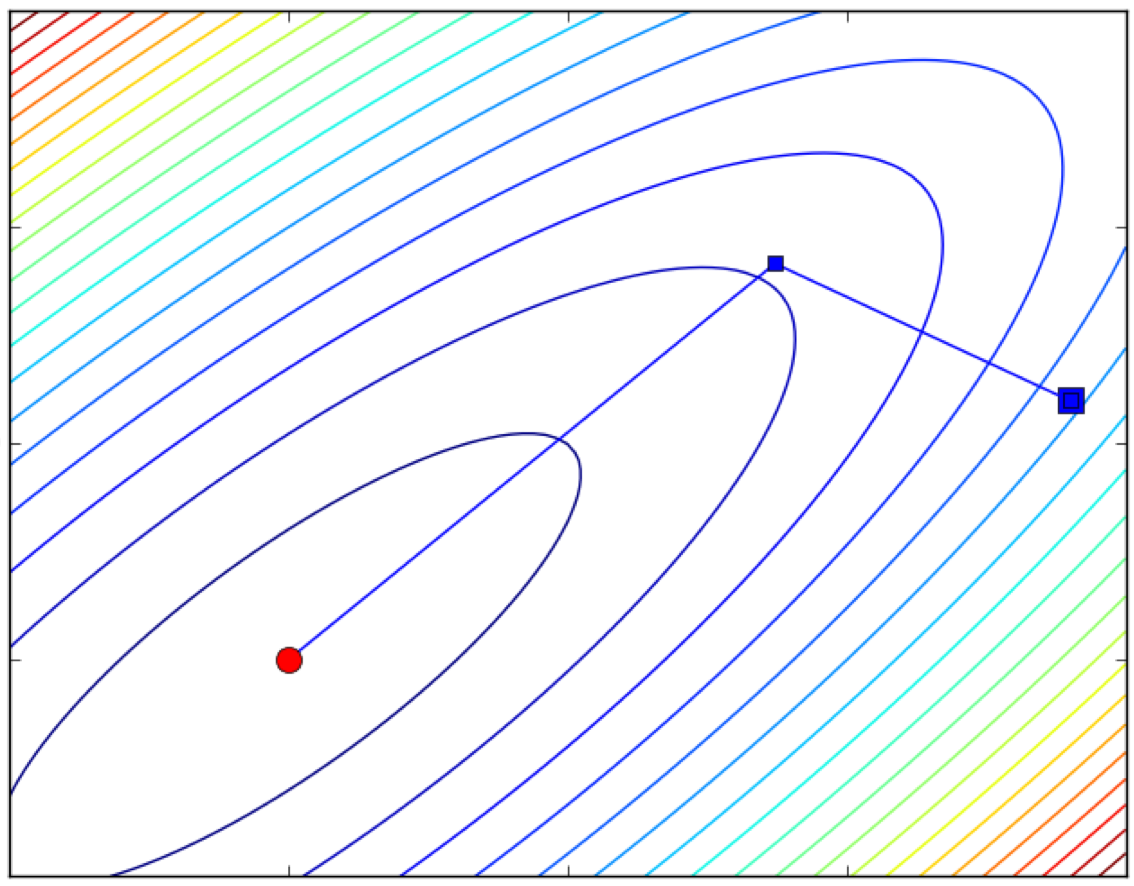
\includegraphics[width=38mm]{exConjugateGradient2D}
\end{columns}
\end{frame}

\begin{frame}
	\frametitle{Iterative Regularization}

Consider
$$
	\min_\bfx \| \bfA \bfx - \bfb \|^2
$$
\begin{itemize}
\item
Assume that $\bfA$ has non-trivial null space
\item The matrix $\bfA^{\top}\bfA$ is not invertible
\item Can we still use iterative methods (CG, CGLS, \ldots)?
\end{itemize}

\bigskip

What are the properties of the iterates? 

\bigskip

Excellent introduction to computational inverse problems~\cite{Hansen1998,Vogel2002,Hansen2010}

\end{frame}




\begin{frame}
	\frametitle{Iterative Regularization: L-Curve}


The CGLS algorithm has the following properties
\begin{itemize}
\item For each iteration $\| \bfA \bfx_j -\bfc \|^2 \le \| \bfA \bfx_{j-1} -\bfc \|^2$
\item If starting from  $\bfx=0$ then $\|\bfx_j  \|^2 \ge \|  \bfx_{j-1}  \|^2$

\item $\bfx_1,\bfx_2,\ldots$ converges to the minimum norm solution of the problem
\item Plotting $\|\bfx_j\|^2$ vs $\| \bfA\bfx_j -\bfc \|^2$ typically has the shape of an L-curve
\end{itemize}



\begin{center}
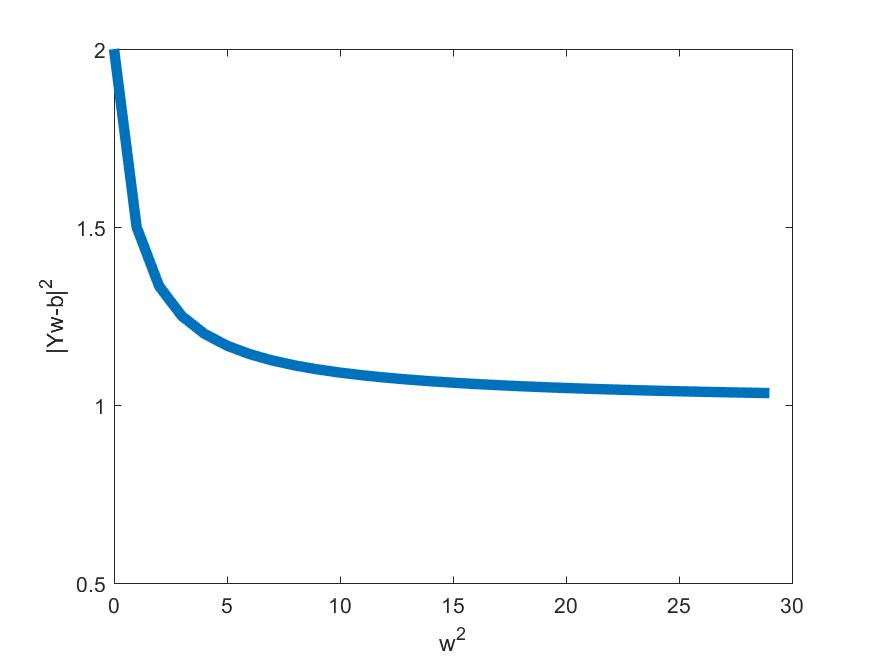
\includegraphics[width=6cm]{lcurve.jpg}
\end{center}

\end{frame}



\begin{frame}[fragile]
	\frametitle{Cross Validation}

Finding good least-squares solution requires good parameter selection.
\begin{itemize}
\item $\lambda$ when using Tikhonov regularization (weight decay)
\item number of iteration (for SD and CGLS)
\end{itemize}

\bigskip

Suppose that we have two different ``solutions''

$$\bfx_1\quad  \rightarrow \quad  \|\bfx_1\|^2 = \eta_1 \quad \|\bfA \bfx_1 - \bfc\|^2 = \rho_1. $$
$$\bfx_2\quad  \rightarrow \quad  \|\bfx_2\|^2 = \eta_2 \quad \|\bfA \bfx_2 - \bfc\|^2 = \rho_2. $$

How to decide which one is better?

\end{frame}

\begin{frame}[fragile]
	\frametitle{Cross Validation}

Measure how well can each of the solutions predict new data.

\bigskip

Let $\{ \bfA_{\rm CV}, \bfc_{\rm CV} \}$ be data that is {\bf not used} for the training 

\bigskip

Then if $\|\bfA_{\rm CV} \bfx_1 - \bfc_{\rm CV}\|^2 \le 
\|\bfA_{\rm CV} \bfx_2 - \bfc_{\rm CV}\|^2$
then $\bfx_1$ is a better solution that $\bfx_2$.

\bigskip

\pause

In general, if the solution depends on some hyper-parameter $\lambda$ then the best one is
$$ \lambda^* = {\rm arg}\min \|\bfA_{\rm CV} \bfx(\lambda) - \bfc_{\rm CV}\|^2. $$

\end{frame}

\begin{frame}[fragile]
	\frametitle{Cross Validation}

To assess the final quality of the solution cross validation is not sufficient (why?).

\bigskip

Need a final testing set.

\bigskip

Procedure
\begin{itemize}
\item Divide the data into 3 groups $\{ \bfA_{\rm train}, \bfA_{\rm CV}, \bfA_{\rm test} \}$.
\item Use $\bfA_{\rm train}$ to estimate $\bfx(\lambda)$
\item Use $\bfA_{\rm CV}$ to estimate $\lambda$
\item Use $\bfA_{\rm test}$ to assess the quality of the solution
\end{itemize}

\pause

{\bf Important} -  we are not allowed to use $\bfA_{\rm test}$ to tune parameters!




\end{frame}




\begin{frame}[fragile]
	\frametitle{Coding: Iterative Methods for Regression}
	
	Outline:
	\begin{itemize}
		\item Dataset: MNIST / CIFAR 10
		\item write a steepest descent specific to the problem
		\begin{verbatim}
			function x = sdLeastSquares(A,c,x0,maxIter)
		\end{verbatim}
		\item write a conjugate gradient code
		\begin{verbatim}
			function x = cgLeastSquares(A,c,maxIter)
		\end{verbatim}
	\end{itemize}
\end{frame}



\begin{frame}[allowframebreaks]
	\frametitle{References}
\bibliographystyle{abbrv}
\bibliography{NumDNN}

\end{frame}
\end{document}
